Yup that's right, we're back with another probability problem
\MarginComment{Probability distributions are just so powerful and interesting
right now, so I'm sorry, but I'm not sorry. I'm taking AP Stats this year, so
this (hopefully, probably won't given AP curriculums) will work well.} inspired
by the beauty of solving the last one. I can't quite make promises one whether
this will be the last one, but I'll try to vary things up now and again
hopefully. I'm planning on making a TODO list entry and as well as a
reading/watch list entry in the near future, so look forward to more writing
based entries :).

As opposed to the previous, explanation-heavy journal entry, I'll likely forego
trying to intuitively explain, detail, and diagram \textit{all} of the
components of the problem because I'm assuming that the reader is at least a
bit more familiar with some of the concepts as they overlap decently with the
previous entry.

With that being said, let's get onto the main problem at hand. Inspired by
previous probability problems, I thought it would be nice to compose another
one involving some interesting geometrical ideas. As such, we have the
following problem:
\begin{blackbox}
    \begin{problem}
        Given two points chosen uniformly randomly from the unit square \(
        \left[ 0, 1 \right]^2 \), what is the expected distance between these
        two points?
    \end{problem}
\end{blackbox}
This time, we seek out not the probability itself, but rather the expected
value, which is a nice little difference from the past problem. I also really
enjoy how innocently the question can be formulated because, as we will come to
see, it's perhaps not the easiest \MarginComment{I've yet to dive head deep in
other solution methods though (the geometric one didn't seem to hopeful), so
perhaps there are other ways of getting the answer?} to solve once you really
take a good think about it.

Initially, this was inspired by a slightly harder probability problem
\MarginComment{Guys, I think he might like probability just a little bit.},
which has a slightly longer formulation and seems to be a decent bit harder,
but I do intend to tackle it someday (and perhaps I might add it at the end of
this journal entry).

\subsection{Non-Probabilistic Methods}

\subsubsection{Brute Forcing, Mathematically}

One of the first methods I tried was applying some good old calculus to the
problem. In particular, if one were to evaluate the following integral
\[
    D = \int\displaylimits_{\left[ 0, 1 \right]^2} \int\displaylimits_{\left[ 0, 1 \right]^2} \norm{\bvec{w} - \bvec{v}} \, d\bvec{w} \, d\bvec{v}
    = \int_{0}^{1} \int_{0}^{1} \int_{0}^{1} \int_{0}^{1} \sqrt{\left( x_2 - x_1 \right)^2 + \left( y_2 - y_1 \right)^2} \, dy_2 \, dx_2 \, dy_1 \, dx_1
.\]
In effect, this is "brute forcing" the answer. We go through each point in the
unit square, and for this point, we go through the unit square once more and
sum all the distances. Because the area of the unit square is simply one, we
don't divide anything and are left with the average, or expected, value of the
distance. The reader might now be thinking: "Ok Rushil, we have our integral,
so why can't I just plug this into Mathematica and go on with my day?"

There's just a slight problem. I too had this train of thought, and I happily
plugged the integral into Mathematica, eager to see what result would come out.
Unfortunately though, \MarginComment{My laptop certainly isn't a Gamer PC\texttrademark, so
there is a chance that it could do it on somebody else's computer, but
given how daunting the integral looks to approach, I severely doubt it.} this
is a quadruple integral, and a painful one to evaluate at that given the square
root. I let the program run until the jet engines noises start coming from my
laptop fans, but it seems this integral is just far too difficult to evaluate
in general, even for a computer using (what I presume to be at least) a
modified Risch algorithm.

That's not to say that this doesn't yield us any information though. Either
through Monte Carlo simulations or some numerical integration using trusty old
SciPy, we do know that
\[
    D \approx 0.521405
,\]
which at the very least intuitively makes some loose sense. This also gives us
a good way to check that our closed form answer is correct whenever we're
trying out another solution.

\subsubsection{A Small Aside on Calculus}

One rather interesting thing to remark about this approach, though, is that the
expected squared distance,
\[
    L = \int\displaylimits_{\left[ 0, 1 \right]^2} \int\displaylimits_{\left[ 0, 1 \right]^2} \norm{\bvec{w} - \bvec{v}}^2 \, d\bvec{w} \, d\bvec{v}
    = \int_{0}^{1} \int_{0}^{1} \int_{0}^{1} \int_{0}^{1} \left[ \left( x_2 - x_1 \right)^2 + \left( y_2 - y_1 \right)^2 \right] \, dy_2 \, dx_2 \, dy_1 \, dx_1
,\]
is actually quite trivial to calculate using this approach. The quadruple
integral is rather easy to evaluate as the following will show, which just
speaks for how the square root alone complicates things massively.
\begin{align*}
    L &= \int_{0}^{1} \int_{0}^{1} \int_{0}^{1} \int_{0}^{1} \left[ \left( x_2 - x_1 \right)^2 + \left( y_2 - y_1 \right)^2 \right] \, dy_2 \, dx_2 \, dy_1 \, dx_1 \\
    &= \int_{0}^{1} \int_{0}^{1} \left[ \frac{1}{3} \left( \left( 1 - x_1 \right)^3 + x_1^3 \right) + \frac{1}{3} \left( \left( 1 - y_1 \right)^3 + y_1^3 \right) \right] \, dy_1 \, dx_1 \\
    &= \int_{0}^{1} \int_{0}^{1} \left[ \frac{1}{3} \left( 1 - 3x_1 + 3x_1^2 \right) + \frac{1}{3} \left( 1 - 3y_1 + 3y_1^2 \right) \right] \, dy_1 \, dx_1 \\
    &= \frac{2}{3} \left( 1 - \frac{3}{2} + 1 \right) \\
    &= \frac{1}{3}
.\end{align*}
At the very least, this potentially gives ourselves another way to check our
work in the future, and it's simply just interesting to think about how
different norms impact the result vastly.

\subsubsection{Some Attempted Geometry}

Another way one might tackle the problem is to look at some geometrical
simplification, trying to utilize symmetries and the like to figure out some
information. Unfortunately, this didn't seem to yield very many useful results
for me, with no real hope of a solution in closed form.

If one draws out the unit square, we can pick a point anywhere in its interior
and then radiate circles outwards at increasing radii in a way not too far from
the brute force integral. We can additionally use symmetry to only consider
points in of the corners of the square (if we rotate/reflect, we can always
transform the square to get a point anywhere in one of the corners while
preserving distances). In total, this works fine for relatively smaller radii,
but as one gets to the circle intersection with the square, everything
complicates, and one is unlikely to get a clean looking closed form solution.

\begin{figure}
    \centering
    \begin{tikzpicture}
        \draw[semithick] (0, 0) -- (0, 3) -- (3, 3) -- (3, 0) -- cycle;

        \fill (0.75, 1.25) circle (0.05);

        \foreach \i in {1, 2, ..., 7} {
            \draw (0.75, 1.25) circle (\i * 0.10);
        }

        \draw[fadegray, thick] (0.75, 1.25) circle (0.8);

        \draw[<-, domain=-157:45, thick, white, smooth] plot ({1.5 + 0.7906 * cos(\x)}, {1.5 + 0.7906 * sin(\x)});
        \draw[<-, domain=-157:45, smooth] plot ({1.5 + 0.7906 * cos(\x)}, {1.5 + 0.7906 * sin(\x)});

        \fill ({1.5 + 0.7906 / sqrt(2)}, {1.5 + 0.7906 / sqrt(2)}) circle (0.05);
    \end{tikzpicture}
    \caption{A diagram illustrating an attempted geometric solution.}
\end{figure}


\subsection{Detectably Delicious Distributions}

And such comes the time where we, stranded travelers on our journey through
this puzzle, are enlightened by the beauty of the probability distributions. As
opposed to straight brute force, I like to think of probability distributions
as a more elegant way of encoding the problem (although they are in some ways
brute force).

The basic plan for our probability distribution approach is that we will build
up the norm, \( \sqrt{\left( X_2 - X_1 \right)^2 + \left( Y_2 - Y_1 \right)^2}
\), using random variables described by distributions as opposed to regular old
scalars. We know that all the coordinate components are uniformly distributed
on \( \left[ 0, 1 \right] \), so it becomes a matter of combining these in a
way that we can get the distribution of the lengths found on the unit square. We will achieve this with the following steps:
\begin{enumerate}
    \item First, convolve our two uniform distributions to find \( T = X_2 - X_1
        \). The support of this distribution should be \( \left[ -1, 1 \right] \).
    \item Next, take the distribution of the squares of the these \( x \)-differences to get \( Q = T^2 = \left( X_2 - X_1 \right)^2 \). The support of this distribution should be \( \left[ 0, 1 \right] \).
    \item Take the convolution of the resulting \( Q \) with itself (as the
        other part of the norm is the exactly the same) to get \( Z = Q + Q =
        \left( X_2 - X_1 \right)^2 + \left( Y_2 - Y_1 \right)^2 \). The support
        fo this distribution should be \( \left[ 0, 2 \right] \), and a good
        check that we have the distribution right is that the mean should be \(
        1 / 3 \), according to our aside above.
    \item To finish off the algebra on our distribution, we'll take the
        distribution of the square roots of the previous \( Z \).
        Intuitively, this should have the support \( \left[ 0, \sqrt{2} \right]
        \), as the greatest possible distance between two points on the unit
        square is the distance between two opposite corners. If all goes well,
        we'll be able to integrate and get the mean of the distribution, which
        will be the expected value of the distance between any two random
        points on the unit square.
\end{enumerate}

With our mental roadmap laid out for us, let's get on with the probability
distributions!

\subsubsection{Opposing Convolutions}

The first step on our special soup distribution \MarginComment{I bet the
distributions are delectably delicious.} recipe is to take the difference of
two uniform distributions spread across the interval \( \left[ 0, 1 \right] \).
Equivalently, this is same as taking the convolution of the aforementioned
uniform distribution with the negative of the same distribution.
\MarginComment{Essentially, \( X - Y = X + \left( -Y \right) \).} In
particular, let \( X_2 \distributed \Uniform{0}{1} \) and \( X_1 \distributed
\Uniform{-1}{0} \). We then desire the distribution \( X_2 + X_1 \), which we
can find by convolving the two distribution PDFs.

In this case, carrying out the convolution just visually is possible as the
overlapping area between the two uniform distributions increases or decreases
linearly as you slide one across another, but we may also verify our results formally. If we write our distributions out as functions, we get
\begin{figure}
    \centering
    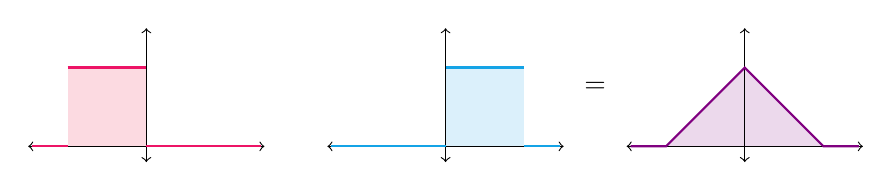
\begin{tikzpicture}
        \fill[WildStrawberry!15] (-1, 1) -- (0, 1) -- (0, 0) -- (-1, 0) -- cycle;

        \draw[<->] (-1.5, 0) -- (1.5, 0);
        \draw[<->] (0, -0.2) -- (0, 1.5);

        \draw[WildStrawberry, thick] (-1, 1) -- (0, 1);
        \draw[WildStrawberry, thick] (-1.45, 0) -- (-1, 0);
        \draw[WildStrawberry, thick] (0, 0) -- (1.45, 0);

        \node at (1.90, 0.75) {\( \convolution \)};

        \fill[Cerulean!15] (3.8, 1) -- (4.8, 1) -- (4.8, 0) -- (3.8, 0) -- cycle;

        \draw[<->] (2.3, 0) -- (5.3, 0);
        \draw[<->] (3.8, -0.2) -- (3.8, 1.5);

        \draw[Cerulean, thick] (3.8, 1) -- (4.8, 1);
        \draw[Cerulean, thick] (2.35, 0) -- (3.8, 0);
        \draw[Cerulean, thick] (4.8, 0) -- (5.25, 0);

        \node at (5.7, 0.75) {\( = \)};

        \fill[Purple!15] (6.6, 0) -- (7.6, 1) -- (8.6, 0) -- cycle;

        \draw[<->] (6.1, 0) -- (9.1, 0);
        \draw[<->] (7.6, -0.2) -- (7.6, 1.5);

        \draw[Purple, thick] (6.15, 0) -- (6.6, 0) -- (7.6, 1) -- (8.6, 0) -- (9.05, 0);
    \end{tikzpicture}
    \caption{When we take the convolution of the two uniform distributions, we get a "unit triangle" around \( x = 0 \).}
\end{figure}

\begin{multicols}{2}
    \[
        f_{X_1} \left( x \right) = \begin{cases}
            1, & \text{for } x \in \left[ -1, 0 \right] \\
            0, & \text{otherwise}
        \end{cases}
    ,\]

    \[
        f_{X_2} \left( x \right) = \begin{cases}
            1, & \text{for } x \in \left[ 0, 1 \right] \\
            0, & \text{otherwise}
        \end{cases}
    .\]
\end{multicols}
\MarginComment{The notation \( f_X \) and \( F_X \) are going to be used
throughout here to denote the PDF and CDF of \( X \) respectively.} With this,
we can find the density function for the resulting distribution through the
integral definition of convolution:
\begin{align*}
    f_{X_2 + X_1} \left( t \right) &= \int_{-\infty}^{\infty} f_{X_2} \left( x \right) f_{X_1} \left( t - x \right) \, dx \\
    &= \int_{0}^{1} f_{X_1} \left( t - x \right) \, dx
.\end{align*}
Using our visual intuition of sliding the distribution of \( X_1 \) along the
\( x \)-axis and seeing the intersecting area with the distribution of \( X_2
\), there are two cases we need to look at:
\begin{enumerate}
    \item \textbf{Case \( x \in \left[ -1, 0 \right] \)}:
    In this case, the area of the sum of the distributions is increasing as the
    two distributions overlap more and more. At \( x = 0 \), they are
    completely on top of each other. This part of the distribution should be
    \[
        f_{X_2 + X_1} \left( t \right) = \int_{0}^{1 + t} \, dx = 1 + t
    .\]

    \item \textbf{Case \( x \in \left( 0, 1 \right] \)}:
    In this case, the area of the sum of the distributions is decreasing as
    they steadily move away from each other, with \( x = 1 \) marking the point
    at which there is again no interlap. This component is given by
    \[
        f_{X_2 + X_1} \left( t \right) = \int_{t}^{1}  \, dx = 1 - t
    .\]
\end{enumerate}

With this, our first step of the distribution recipe is completed. We have the following distribution representing the difference between components:
\[
    f_T \left( t \right) = \begin{cases}
        1 + t, & \text{for } t \in \left[ -1, 0 \right] \\
        1 - t, & \text{for } t \in \left( 0, 1 \right] \\
        0, & \text{otherwise}
    \end{cases}
.\]
The next step in our cooking journey will be to take the distribution of the
squares of \( T \).

\subsubsection{A Not So Square-Looking Square}

As mentioned, we're looking for a probability distribution that tells gives us the distribution of the squares of \( T \). Intuitively, this should have \( 0 \) probability for all values less than \( 0 \) or greater than \( 1 \). We are able to find this distribution by looking at the CDF of \( T^2 \) and \( T \). One has
\[
    \Prob{T^2 \leqslant t} = \Prob{T \in \left[ -\sqrt{t}, \sqrt{t} \right]} = 2 \Prob{T \in \left[ 0, \sqrt{t} \right]}
.\]
In short, we have the CDF of \( T^2 \) in terms of the CDF of \( T \), and
because we can find the CDF of \( T \) given the PDF of \( T \) quite easily,
we're able to get our desired distribution for \( T^2 \) with just a little bit
of work. The above relations tell us that
\begin{align*}
    F_{T^2} \left( t \right) &= 2\int_{0}^{\sqrt{t}} f_T \left( x \right) \, dx \\
    &= 2\int_{0}^{\sqrt{t}} \left( 1 - x \right) \, dx \\
    \implies f_{T^2} \left( t \right) &= 2 \frac{d}{dt} \int_{0}^{\sqrt{t}} \left( 1 - x \right) \, dx
.\end{align*}
Note that we were able to only use the positive component of the distribution
of \( T \) due to its symmetry across \( x = 0 \). Now applying a little bit of the fundamental theorem of calculus, we get a decently reasonable expression for the PDF of \( T^2 \).
\[
    f_{T^2} \left( t \right) = f_{Q} \left( t \right) = \frac{1}{\sqrt{t}} - 1
.\]
This distribution is quite an interesting one (see Figure \ref{013:tsquared}),
as it approaches infinity as \( t \to 0^+ \) and it hits \( 0 \) at \( t = 1
\).
\begin{figure}
    \centering
    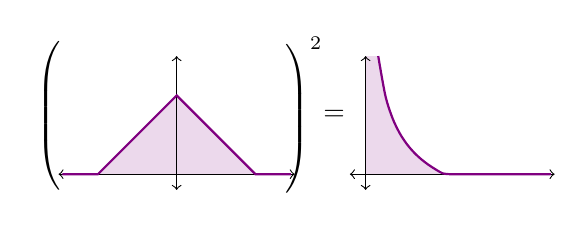
\begin{tikzpicture}
        \fill[Purple!15] (-1, 0) -- (0, 1) -- (1, 0) -- cycle;

        \draw[<->] (-1.5, 0) -- (1.5, 0);
        \draw[<->] (0, -0.2) -- (0, 1.5);

        \draw[Purple, thick] (-1.45, 0) -- (-1, 0) -- (0, 1) -- (1, 0) -- (1.45, 0);

        \node at (-1.6, 0.75) {\( \left(\rule{0pt}{30pt} \right. \)};
        \node at (1.6, 0.75) {\( \left. \rule{0pt}{30pt} \right)^2 \)};

        \node at (2.0, 0.75) {\( = \)};

        \fill[color=Purple!15, thick, domain=0.16:1] plot ({\x + 2.4}, {1/sqrt(\x) - 1}) -- (2.4,0) -- (2.4, 1.5) -- cycle;

        \draw[<->] (2.2, 0) -- (4.8, 0);
        \draw[<->] (2.4, -0.2) -- (2.4, 1.5);

        \draw[Purple, thick] (3.4, 0) -- (4.75, 0);
        \draw[color=Purple, thick, domain=0.16:2.35, smooth] plot ({\x + 2.4}, {(1/sqrt(\x) - 1) * (\x <= 1) + (\x > 1) * (0)});
    \end{tikzpicture}
    \caption{The distribution of the squares of the differences in components.
    It looks rather interesting as it approaches infinity on one side.}
    \label{013:tsquared}
\end{figure}

With this, we have our second step of our recipe done, and we're almost halfway
to the goal. In the next section, we'll need to take this distribution and
convolve it with itself once more.

\subsubsection{More Beautiful Convolutions}

Once more we must take the convolution of this distribution with itself. Unlike
how the case was with the uniform distribution convolutions, though, this is a
bit more to work through especially given that the distributions are no longer
described by simple functions. Once again, we'll have to use our visual
intuition to split the domain into separate cases.

Using the convolution formula once again, we have
\begin{align*}
    f_{Q+Q} \left( q \right) &= \int_{0}^{1} f_Q \left( x \right) f_Q \left( q - x \right) \, dx \\
    &= \int_{0}^{1} \left( \frac{1}{\sqrt{x}} - 1 \right) f_Q \left( q - x \right) \, dx
.\end{align*}
We once again must split this case-wise based on \( q \):
\begin{enumerate}
    \item \textbf{Case \( q \in \left[ 0, 1 \right] \)}:
    For this case, the lower bound is \( 0 \) and the upper bound is \( q \).
    This gives us
    \[
        f_{Q+Q} \left( q \right) = \int_{0}^{q} \left( \frac{1}{\sqrt{x}} - 1 \right) \left( \frac{1}{\sqrt{q - x}} - 1 \right) \, dx
    .\]


    \item \textbf{Case \( q \in \left[ 1, 2 \right] \)}:
    In this case, the lower bound is \( q - 1 \) and the upper bound shall be
    \( 1 \).
    \[
        f_{Q+Q} \left( q \right) = \int_{q - 1}^{1} \left( \frac{1}{\sqrt{x}} - 1 \right) \left( \frac{1}{\sqrt{q - x}} - 1 \right) \, dx
    .\]
\end{enumerate}
In order to not repeat ourselves and do too much work, we'll find the general
antiderivative of the shared integrand between these two cases. Expanding yields the following
\begin{align*}
    \int \left( \frac{1}{\sqrt{x}} - 1 \right) \left( \frac{1}{\sqrt{q - x}} - 1 \right) \, dx &= x - 2 \sqrt{x} + 2 \sqrt{q - x} + \int \frac{1}{\sqrt{x} \sqrt{q - x}} \, dx \\
    &= \cdots + 2\int \frac{1}{\sqrt{q - u^2}} \, du \\
    &= \cdots + \frac{2}{\sqrt{q}} \int \frac{1}{\sqrt{1 - \left( \frac{u}{\sqrt{q}} \right)^2}} \, du \\
    &= x - 2 \sqrt{x} + 2 \sqrt{q - x} + 2 \arcsin{\left( \frac{\sqrt{x}}{\sqrt{q}} \right)} + C
\end{align*}
So, for the first case, the distribution looks something like \( \pi - 4
\sqrt{q} + q \), and the second case will be something like \( 4 \sqrt{q - 1} -
y - 2 + \pi - \arctan{\left( \sqrt{y - 1} \right)} \). \MarginComment{This is
achieved using the relation \( \arctan{x} = \arcsin{(x / \sqrt{1 - x^2})} \).
While one can proceed with using \( \arcsin \), flipping to \( \arctan \) makes
future integration much easier.} Written in a more convenient form, we get the
full distribution to be something like
\[
    f_{Q+Q} \left( q \right) = \begin{cases}
        \pi - 4\sqrt{q} + q, & \text{for } q \in \left[ 0, 1 \right] \\
        \pi - q - 2 - 4\arctan{\left( \sqrt{q - 1} \right)} + 4\sqrt{q - 1}, & \text{for } q \in \left( 1, 2 \right]
    \end{cases}
.\]
This distribution in fact does \textit{not} approach infinity as \( q \to 0^+
\), and looks rather interesting, although similar in shape to the distribution
for \( Q \). \MarginComment{
    \begin{center}
    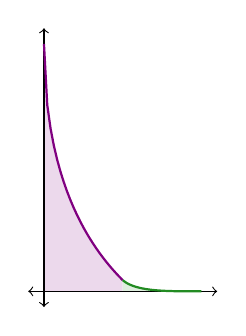
\begin{tikzpicture}
        \fill[color=Purple!15, thick, domain=0:1] plot (\x, {pi - 4 * sqrt(\x) + \x}) -- (1, 0) -- (0, 0) -- cycle;
        \fill[color=ForestGreen!15, thick, domain=1:2] plot (\x, {pi - \x - 2 - 4 * rad(atan(sqrt(\x - 1))) + 4 * sqrt(\x - 1)}) -- (1, 0) -- cycle;

        \draw[<->] (-0.2, 0) -- (2.2, 0);
        \draw[<->] (0, -0.2) -- (0, 3.3415);

        \draw[color=Purple, thick, domain=0:1] plot (\x, {pi - 4 * sqrt(\x) + \x});
        \draw[color=ForestGreen, thick, domain=1:2] plot (\x, {pi - \x - 2 - 4 * rad(atan(sqrt(\x - 1))) + 4 * sqrt(\x - 1)});
    \end{tikzpicture}
\end{center}
\captionof{figure}{The distribution of the squared distances. It looks rather odd in a way, and the presence of \( \pi \) terms seems quite interesting.}

}
Indeed a good check that we're on the right path is showing that
\[
    \int_{0}^{2} z f_{Z} \left( z \right) \, dz = \frac{1}{3}
,\]
which we found in the non-probabilistic solution attempts section. Now all
that's left to do is take the distribution of the square roots, and we'll be
able to integrate to find the mean and our desired answer.

\subsubsection{The Last Stretch and Some Fancy Integrals}

Doing something similar to the squaring section, we'll take a look at the CDFs
of \( \sqrt{Z} \) and \( Z \) and find a relation between them, which will
allow us to get the final distribution. In particular, \MarginComment{\begin{center}
    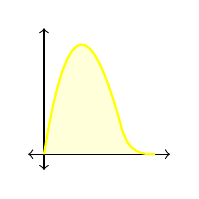
\begin{tikzpicture}
        \fill[color=Yellow!15, thick, domain=0:1.412136] plot (\x, {(\x <= 1) * (2 * pi * \x - 8 * \x^2 + 2 * \x^3) + (\x > 1) * (2 * pi * \x - 2 * \x^3 - 4 * \x + 8 * \x * sqrt(abs(\x^2 - 1)) - 8 * \x * rad(atan(sqrt(abs(\x^2 - 1)))))}) -- (0, 0) -- cycle;

        \draw[<->] (-0.2, 0) -- (1.6, 0);
        \draw[<->] (0, -0.2) -- (0, 1.6);

        \draw[color=Yellow, thick, domain=0:1.412136] plot (\x, {(\x <= 1) * (2 * pi * \x - 8 * \x^2 + 2 * \x^3) + (\x > 1) * (2 * pi * \x - 2 * \x^3 - 4 * \x + 8 * \x * sqrt(abs(\x^2 - 1)) - 8 * \x * rad(atan(sqrt(abs(\x^2 - 1)))))});
    \end{tikzpicture}
\end{center}
\captionof{figure}{The final distribution and the distribution of all distances
between two points found on the unit square. This particular distribution has a
somewhat intuitive shape. Note however that the mean is not the extreme value,
although they look somewhat close.}
}
\begin{align*}
    F_{\sqrt{Z}} \left( z \right) &= \Prob{\sqrt{Z} \leqslant z} = \Prob{Z \leqslant z^2} = F_{Z} \left( z^2 \right) \\
    \implies f_{\sqrt{Z}} \left( z \right) &= \frac{d}{dz} \int_{0}^{z^2} f_Z \left( x \right) \, dx = 2z f_Z \left( z^2 \right)
.\end{align*}
We want to take the mean of this distribution, which can be found using
\[
    \int_{0}^{\sqrt{2}} z f_{\sqrt{Z}} \left( z \right) \, dz = 2 \int_{0}^{\sqrt{2}} z^2 f_Z \left( z^2 \right) \, dz
.\]
This once again must be split into two cases given the piecewise nature of the
function, and now we have some nice integrals to evaluate.
\begin{align*}
    &= \int_{0}^{1} \left( 2 \pi z^2 - 8z^3 + 2z^4 \right) \, dz \\
    &+ \int_{1}^{\sqrt{2}} \left( 2 \pi z^2 - 4z^2 - 2z^4 + 8z^2 \sqrt{z^2 - 1} - 8z^2 \arctan{\left( \sqrt{z^2 - 1} \right)} \right) \, dz
.\end{align*}
The first integral is easy enough to evaluate, and I'll cut straight to the
simplification for that one, but two of the terms in the last integral aren't
as trivial to integrate in one's head, so we'll focus on those. Before moving
on, let's prove the following useful result for future use.
\begin{lemma}
    \[
        \int \sec^n{\theta} \, d\theta = \frac{1}{n - 1} \sec^{n - 2}{\theta} \tan{\theta} + \frac{n - 2}{n - 1} \int \sec^{n-2}{\theta} \, d\theta
    .\]
\end{lemma}
\begin{proof}
    Using integration by parts, take
    \begin{align*}
        u = \sec^{n-2}{\theta} \quad &du = \left( n - 2 \right) \sec^{n-2}{\theta} \tan{\theta} \, d\theta \\
        dv = \sec^2{\theta} \, d\theta \quad &v = \tan{\theta}
    \end{align*}
    This gives us
    \begin{align*}
        \int \sec^n{\theta} \, d\theta &= \sec^{n-2}{\theta} \tan{\theta} - \left( n - 2 \right) \int \left( \sec^{n}{\theta} - \sec^{n-2}{\theta} \right) \, d\theta \\
        \implies \left( n - 1 \right) \int \sec^{n}{\theta} \, d\theta &= \sec^{n-2}{\theta} \tan{\theta} + \left( n - 2 \right) \int \sec^{n-2}{\theta} \, d\theta \\
        \implies \int \sec^{n}{\theta} \, d\theta &= \frac{1}{n - 1} \sec^{n-2}{\theta} \tan{\theta} + \frac{n - 2}{n - 1} \int \sec^{n-2}{\theta} \, d\theta
    .\end{align*}
    Thus completes the proof.
\end{proof}
Now that this nice tool at our disposal, we can go ahead and tackle the two "non-trivial" integrals in the expression:
\begin{enumerate}
    \item For the first integral we can do a trig substitution, setting \( z = \sec{\theta} \) to yield
    \begin{align*}
        &\int_{1}^{\sqrt{2}} 8z^2 \sqrt{z^2 - 1} \, dz \\
        &= 8 \int_{1}^{\sqrt{2}} \sec^3{\theta} \tan^2{\theta} \, d\theta \\
        &= 8 \int_{0}^{\pi / 4} \left( \sec^5{\theta} - \sec^3{\theta} \right) \, d\theta \\
        &= 4 \sqrt{2} - \sqrt{2} + \ln{\left( 1 + \sqrt{2} \right)} \\
        &= 3 \sqrt{2} + \ln{\left( 1 + \sqrt{2} \right)}
    .\end{align*}

    \item For the second integral, we can use IBP to differentiate the \( \arctan \) term and integrate the polynomial term to get
    \begin{align*}
        &\int_{1}^{\sqrt{2}} 8z^2 \arctan{\left( \sqrt{z^2 - 1} \right)} \, dz \\
        &= \frac{4 \sqrt{2} \pi}{3} - \frac{8}{3} \int_{1}^{\sqrt{2}} \frac{z^2}{\sqrt{z^2 - 1}} \, dz \\
        &= \frac{4 \sqrt{2} \pi}{3} - \frac{8}{3} \int_{0}^{\pi / 4} \sec^3{\theta} \, d\theta \\
        &= \frac{4 \sqrt{2} \pi}{3} - \frac{4}{3} \left( \sqrt{2} + \ln{\left( 1 + \sqrt{2} \right)} \right) \\
        &= \frac{4 \sqrt{2} \pi}{3} - \frac{4 \sqrt{2}}{3} - \frac{4}{3} \ln{\left( 1 + \sqrt{2} \right)}
    .\end{align*}
\end{enumerate}
Now that we have these results, it becomes a matter of combining terms and
simplifications, which I won't bore you too much with. After we cancel a couple
of terms down, \MarginComment{One can also write the logarithm term in terms of
inverse hyperbolic sine, but that feels a little obfuscated.} we get the
following expression for the average distance between two randomly picked
points on the unit square:
\[
    D = \boxed{\frac{1}{15} \left( 2 + \sqrt{2} + 5 \ln{\left( 1 + \sqrt{2} \right)} \right)}
.\]
Numerically, this does check out with both the brute force integral as well as
the Monte Carlo methods, so we truly do have our final answer. One of the
things that I found most surprising was that the answer doesn't really look all
that clean or intuitive or anything. All of the \( \pi \) terms magically
cleared, so there's no real circles to intuit. Given the nature of the
solution, it really doesn't feel that there is a good geometric way to solve
the problem (and get a closed form at least) as I suspected at the beginning.

This was quite the fun problem!

\subsection{The Aforementioned Parent Problem}

As somewhat mentioned in the introduction, the idea for the problem we just
solved was born alongside a slightly harder problem that I'd like to at least
put down here along with my thoughts. The problem follows as such:
\begin{blackbox}
    \begin{problem}
        Suppose we randomly place \( n \) points on the unit square and number
        these points accordingly \( 1,2,\ldots,n \). In addition, extend lines
        between points \( k \) and \( k + 1 \) for \( k \in \set{1, 2, \ldots, n -
        1} \). What is the probability that none of the edges between the points
        intersect?
    \end{problem}
\end{blackbox}
Certainly, while there are some similarities, it is also a decently different
problem. I have yet to fully tackle this problem (and I have other things that
I would like to work on as well, so it won't be done in the near future), but
at least my main starting point would be to look at the angles formed between
the points. An \( n \)-gon has a certain interior angle sum, and so going along
this thinking, we could create some conditions on the individual angles or the
sum of these angles that leads us in the right direction. Certainly, if an
angle is far to narrow, we might find an intersection. If all angles are
perhaps larger than a certain threshold, we can say for certain that there is
no intersection.

In addition, as a general problem solving tip, it will help to look at smaller
cases. One can easily see that for \( n \leqslant 3 \) \MarginComment{One may
notice for the \( n = 3 \) case there is a line segment of points where we
can place the third point which folds back upon the first point, but this
realistically has zero measure, so it doesn't contribute (at least I think).}
has a probability of \( 1 \) for there being no intersections. From there, we
can build up our geometric intuition of the problem.

I look forward to seeing what sort of form both the solution
structure as well as the closed form answer (assuming there is one) takes on.

